\chapter{High Level}

\section{Overview}
The goal of the following chapter is to describe the high level functionality of the whole system. The kidnapped robot problem is still quite an open issue in the Robotic Community and consequently the solution presented is quite conceptual. To tackle the problem the functionality has been divided into two main parts. The first one is detection of the kidnapping situation and the second one is recovery from this state. Information sources available for these tasks consist of MCA odometry and laser data, data from Kinect and finally fused data from Extended Kalman Filter. The pose information can be obtained from EKF which merges the result from Kalman Filter in MCA and the output from Kinect. The data from odometry and laser scanner can be acquired through MCA. 

The structure of the whole system is shown in Figure \ref{System}. Section \ref{implementation} provides information about implementation of detection and recovery tasks. It describes interaction with other modules of the project and the concepts of actions taken by the robot itself. Section \ref{problems} describes problems and difficulties met mainly during testing process.

\begin{figure}[ht]
\centering
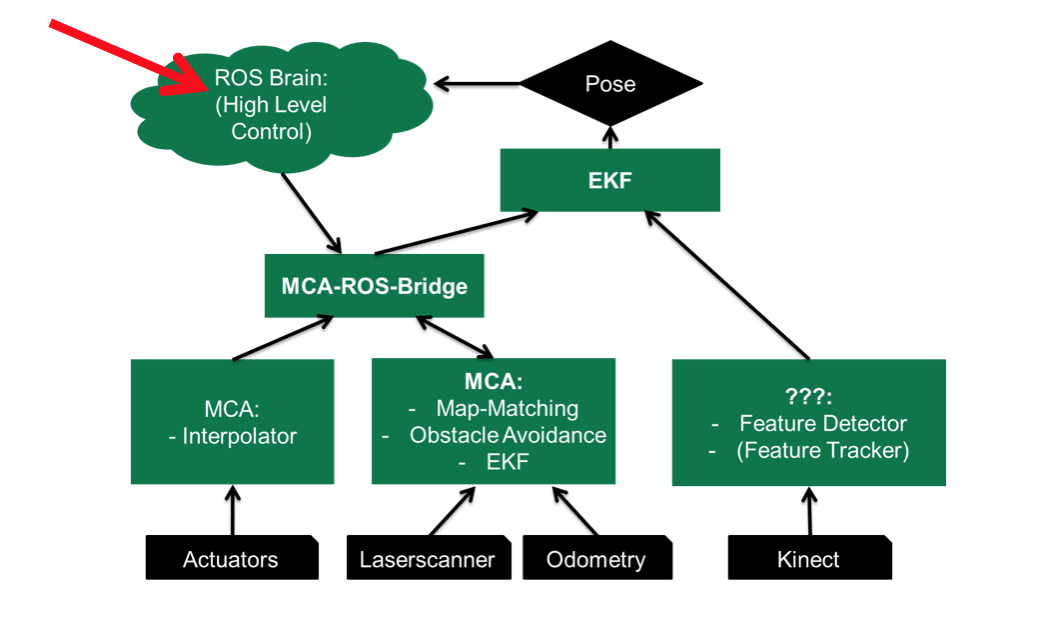
\includegraphics[width=0.9\textwidth]{graphics/system.png}
\caption{Overview of the system}
\label{System}
\centering
\end{figure}

\section{Implementation} \label{implementation}
\subsection{Detection}
The detection was the first step used to solve the problem and was realized inside of the \texttt{kidnap\_detection} node of ROS. 

\subsubsection{Interface}
\begin{description}
\item[List of subscribers]\
	\begin{itemize}
	\item ``/kalman/fused\_pose'' 
	\item ``/vision/unexpected\_marker'' 
	\item ``/poseupdate'' 
	\item ``/HL/is\_kidnapped''
	\end{itemize}
\end{description}

This node communicates through subscribers and publisher listed above. The topic \texttt{/kalman/fused\_pose} delivers the pose fused by Exteded Kalman Filter from MCA and Kinect data. The information about unexpected marker found is delivered as a flag in the topic \texttt{/vision/unexpected\_marker}. The odometry data from the topic \texttt{/poseupdate} deliveres the timestamp needed for calculations. 

\begin{description}
\item[List of publishers]\
	\begin{itemize}
	\item ``/HL/is\_kidnapped''
	\end{itemize}
\end{description}

The flag about kidnap situation in the topic \texttt{/HL/is\_kidnapped} is used for the internal communication of the high level nodes, so it is both published and subscribed by the \texttt{kidnap\_detection} node.

\subsubsection{Concept}
Three criteria were taken into account to detect the kidnap situation: timestamp of odometry, unexpected marker and big covariance.

\begin{itemize}
\item Firstly, the robot regularly compares the current time of odometry data with the timestamp of last message it received from the topic \texttt{/robot/lauron/odom}. The difference between these two timestamps is compared to a certain threshold. Exceeding the threshold means, that the robot has not received data from odometry for a while and is interpreted as kidnapping. The covariance information from the topic \texttt{/kalman/fused\_pose} shall represent that situation in its values since kidnap situation happens with high covariance of the pose. The current variances in x and y directions are then used for setting the threshold stored for the third criterion.
The variance of Yaw is not considered because these data from MCA have large fluctuation and are not reliable for the observation. This is also the reason why the covariance matrix from Kalman Filter on receiving the unexpected marker is saved rather than the timestamps.
\item Secondly, the robot subscribes to the topic \texttt{/vision/unexpected\_marker}. If an unexpected marker is received, it indicates a kidnapping situation (since there is a known map of markers in the global map). Unexpected markers only occur in a situation that the assumed pose by the robot is different from the real pose. If so happens, the covariance information from the topic \texttt{/kalman/fused\_pose} is again stored as the threshold for the third criterion.
\item Thirdly, the robot constantly receives covariance information from the topic
\\
\texttt{/kalman/fused\_pose}. If it suddenly contains values that exceed the saved threshold, it is considered as a kidnapping too.
\end{itemize}

The detection is done at the arrival of some new information. Otherwise, when no new data arrives, the kidnap detection is executed every 2 seconds.
 
In the beginning, we searched for some detection methods in the literature and publications, then finally decided to use the ``strong change of covariance'' as our kidnap detection criterion, which can be represented in a second-order derivative. However, we could only obtain little data from Kalman Filter about a kidnap situation, so it was difficult to define how strong is ``strong'' when working with real data. Therefore, we directly used the covariance matrix. There are still some other methods to achieve the detection such as using the Map-Matching confidence rate or with help of a particle filter.

\subsection{Recovery}
Recovery was the second step used to solve the problem and was realized inside of the
\\
\texttt{kidnap\_recovery} node of ROS. With the help of \texttt{spinner()} , subscription to the topics from other modules and publishing to them could be achieved in parallel using the multithreading feature of \texttt{ROS}. 

\subsubsection{Interface}
\begin{description}
\item[List of subscribers]\
	\begin{itemize}
	\item ``/laser\_vor/scan'' 
	\item ``/laser\_hinter/scan'' 
	\item ``/HL/laser\_data\_obtained''
	\item ``/robot/lauron/odom''
	\item ``/vision/sees\_marker'' 
	\item ``/vision/estimated\_pose'' 
	\item ``/HL/is\_kidnapped'' 
	\item ``/poseupdate'' 
	\item ``/HL/is\_kidnapped'' 
	\end{itemize}
\end{description}	
	
This node communicates through subscribers and publishers listed above. The data from both front and back laser sensors is obtained through topics \texttt{/laser\_vor/scan} and
\\
\texttt{/laser\_hinter/scan} and the flag in the topic \texttt{/HL/laser\_data\_obtained} indicates whether the delivery was successful. Odometry data is obtained from the topic \texttt{/robot/lauron/odom}. The subscriptions to the vision module consist of a topic indicating whether a marker is seen in the environment and another one delivering the pose estimated with Kinect, being \texttt{/vision/sees\_marker} and \texttt{/vision/estimated\_pose} respectively. The topic \texttt{/HL/is\_kidnapped} serves as communication with the detection node. If the robot is kidnapped, the flag is set to true and the subscription callback starts recovery procedure. Due to the fact that calculations in the recovery node are in local coordinate system, \texttt{/HL/is\_kidnapped} is also used to trigger the transformation from world coordinates. After the recovery, the inverse transformation returns the pose in world coordinates again.

\begin{description}	
\item[List of publishers]\
	\begin{itemize}
	\item ``/robot/lauron/cmd\_vel''
	\item ``/HL/laser\_data\_obtained''
	\item ``/HL/is\_kidnapped''
	\item ``/vision/unexpected\_marker''
	\item ``/initialpose''
	\item ``/tf''
	\end{itemize}
\end{description}

The node publishes the twist directly to the robot with the topic \texttt{/robot/lauron/cmd\_vel}. Further, information about successful data delivery from laser sensors is indicated with the topic \texttt{/HL/laser\_data\_obtained}. Robot's initial pose is published as \texttt{/initialpose} and the transformation between local and world coordinate systems as \texttt{/tf}. If an unexpected marker has been detected, it is passed further in the \texttt{/vision/unexpected\_marker} topic, and for internal communication with the detection node as well as for other modules the kidnap state is reported with \texttt{/HL/is\_kidnapped}.

\subsubsection{Concept}
The process of relocalization is triggered if the topic \texttt{/HL/is\_kidnapped} indicates a kidnapping situation. After determining whether the robot is kidnapped, it travels the whole room to search for QR codes or other features thanks to which it can relocalize. The basic concept to achieve this goal is a maze-solving algorithm, which keeps the robot moving on the left side along obstacles. The robot should go over every corner without colliding with obstacles. It achieves this by using the information from laser scanners and odometry. After eventually seeing the marker, the exploration comes to an end and transformation is calculated between frames \texttt{/local\_map} and \texttt{/global\_map}. Considering safety aspects, various driving speeds were defined for the exploration by the robot in different zones, depending on the distances to the obstacles in the environment. The closer the robot is to the obstacle, the slower it is. When the distance between the laser scanner and the obstacle becomes less than 0.11 meter, the robot should stop. When distance is less than 0.3 meter, the robot should move slowly.

The algorithm is implemented as a function \texttt{startRecovery()} and its flow is presented in Figure \ref{start_recovery} with its steps in the following description:

\begin{figure}[ht]
\centering
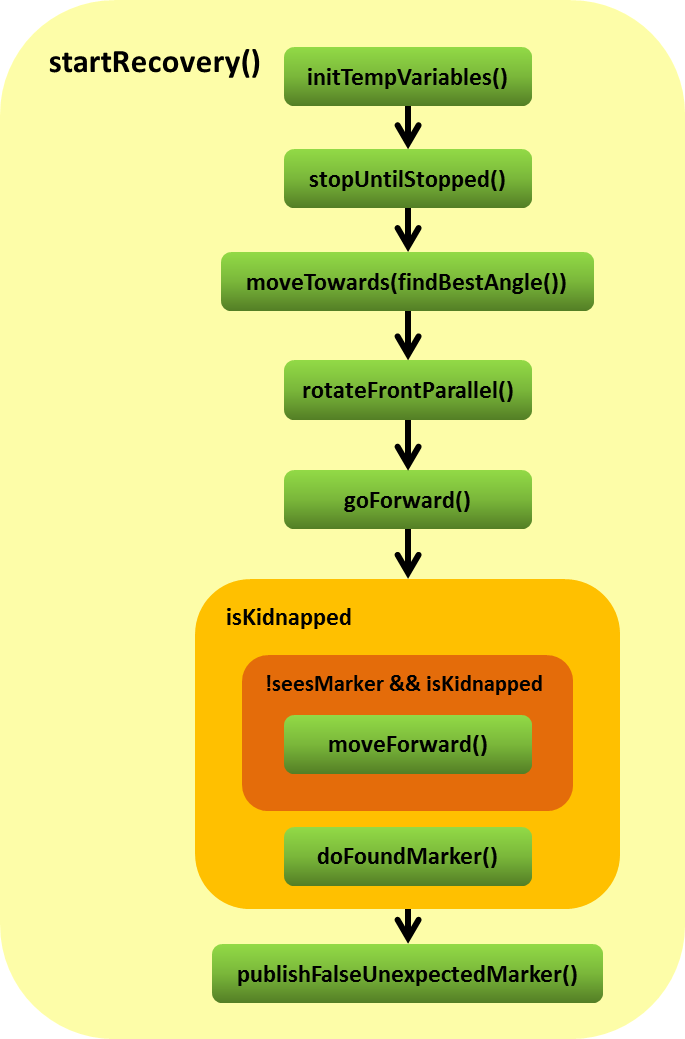
\includegraphics[width=0.7\textwidth]{graphics/start_recovery.png}
\caption{Recovery algorithm}
\label{start_recovery}
\centering
\end{figure}

\begin{description}
\item[initTempVariables()] The function initializes the internal temporary data. 
\item[stopUntilStopped()] The function stops the robot. It is realized by publishing linear and angular twist of the robot as zero. Because a simple publishing would result in the code to continue its execution, the function waits until the robot really stops. The threshold is set so that a negligibly small value of twist is recognized as zero.
\item[lookAround()] The function causes the robot to make the full 360$^{\circ}$ rotation to observe the environment. As shown in Figure \ref{sensor} the front left sensor covers mostly left and front of the robot and can detect the red dots, while the back right sensor covers mainly the right and back of the robot and can detect the blue dots. The regions of overlap can be detected by both sensors. After rotation the robot stops. In the meanwhile, the laser scanners scan environment and save the data with a given sampling rate, ranges being expressed in meters. For the proper format of the data, the angles are normalized. FIXME
\item[moveTowards(findBestAngle())] The function takes as an argument the best found angle and compares with the robot's actual orientation. Robot then rotates to the target angle and goes with the defined velocity \texttt{DEFAULT\_FORWARD\_VELOCITY}
 until it finds itself in the area where it has to slow down, and finally in the distance to the obstacle where it has to stop. The ``speed'' areas are shown in Figure \ref{Zone}, and the thresholds are respectively \texttt{MIN\_FRONT\_DISTANCE} and \texttt{MIN\_CAUTION\_DISTANCE}. 
 Finding the best angle means simply calculating the minimum distance among sampled scans and returning its angle, as shown in Figure \ref{best}, now in millimeters. Due to laser properties negligibly small distances are not considered.
\item[rotateFrontParallel()] The function rotates the robot until it is aligned parallel to the obstacle with its front, as shown in Figure \ref{parallel}. Merged information from both front and back lasers are used. Two points that are spot in front interval of the robot and have the smallest distance are considered a pair from which an average is calculated. That average is treated as a pivot point of the robot rotation. Points which are detected around the pivot are grouped into either left or right side and averaged again. The resulting final left and right average points form a vector to which the robot has to align itself. The averaging adds robustness to the process and tackles the problem of longitudinal inaccuracy of laser scans.
\item[goForward()] The function moves the robot forward with the given \texttt{DEFAULT\_FORWARD\_VELOCITY}.
\item[isKidnapped] The flag indicates whether kidnap situation has been detected, subscribed from the topic \texttt{/HL/is\_kidnapped}.
\item[seesMarker] The flag indicates whether the QR marker was seen by the vision module, subscribed from the topic \texttt{/vision/sees\_marker}.
\item[moveForward()] The function constitutes a core of the recovery algorithm and is described later on.
\item[doFoundMarker()] The function reacts in a situation where a QR marker was seen. It stops for 0.5 seconds and publishes that the robot is not kidnapped anymore.
\item[publishFalseUnexpectedMarker()] The function communicates with the vision module by publishing to the topic \texttt{/vision/unexpected\_marker} that an unexpected marker was seen.
\end{description}

\begin{figure}[ht]
\centering
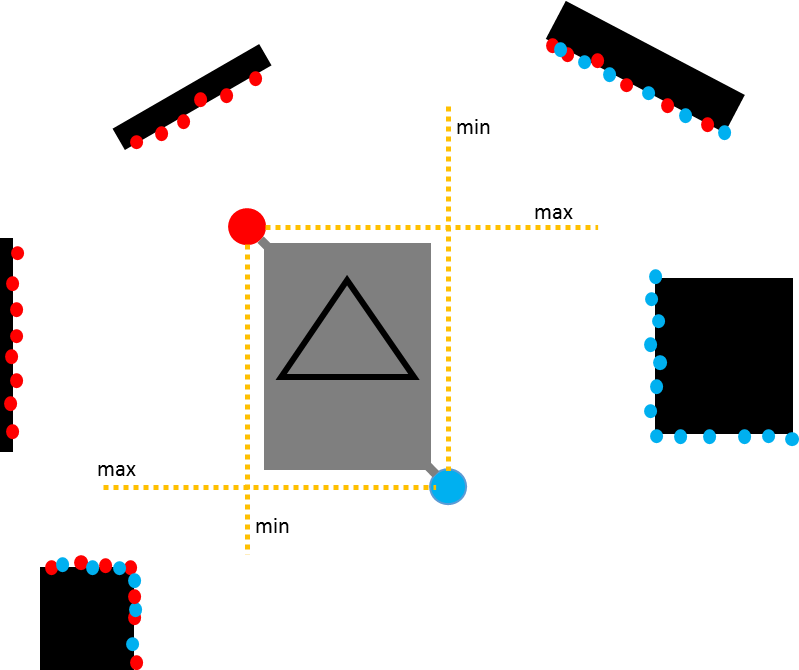
\includegraphics[width=0.7\textwidth]{graphics/sensoren.png}
\caption{Observing of the environment}
\label{sensor}
\centering
\end{figure}

\begin{figure}[ht]
\centering
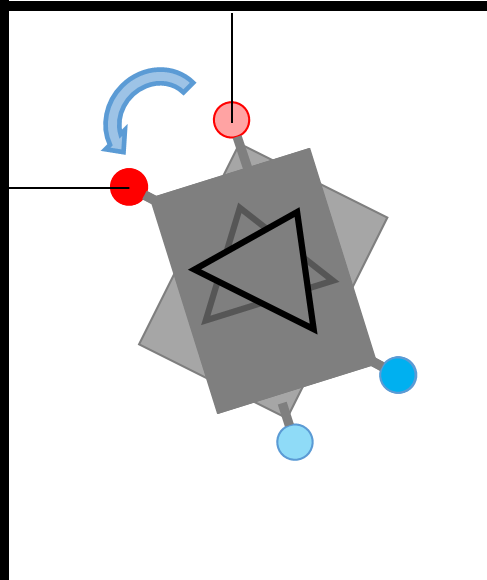
\includegraphics[width=0.5\textwidth]{graphics/find_best_angle.png}
\caption{Finding the best\_angle}
\label{best}
\centering
\end{figure}

\begin{figure}[ht]
\centering
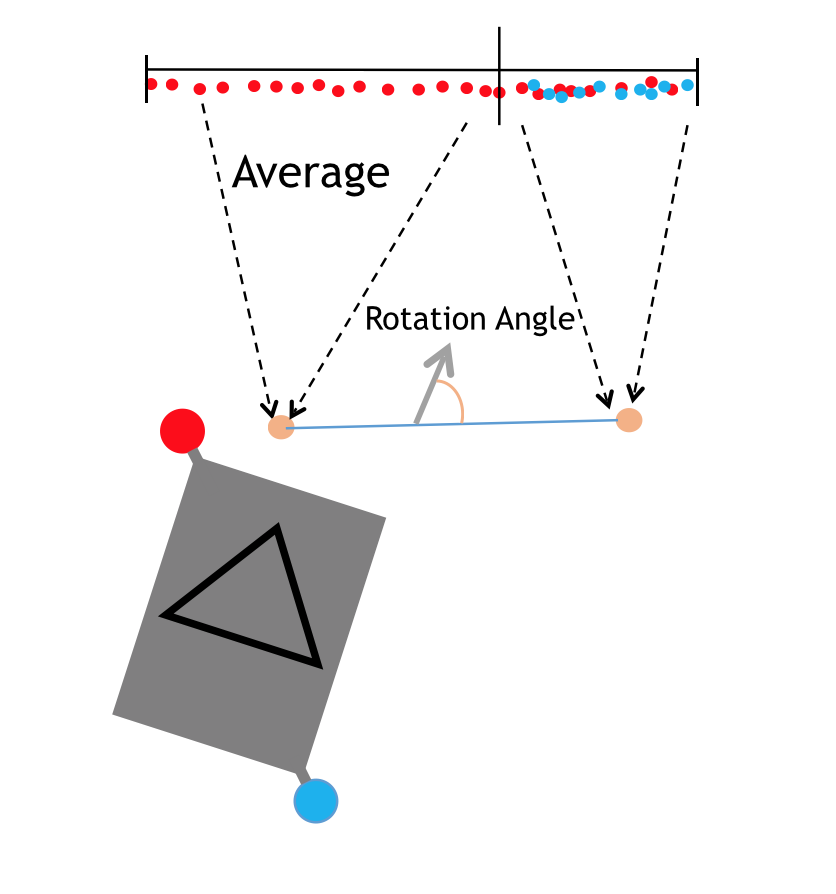
\includegraphics[width=0.5\textwidth]{graphics/front_parallel.png}
\caption{Rotating to align front parallel to the obstacle}
\label{parallel}
\centering
\end{figure}

\begin{figure}[ht]
\centering
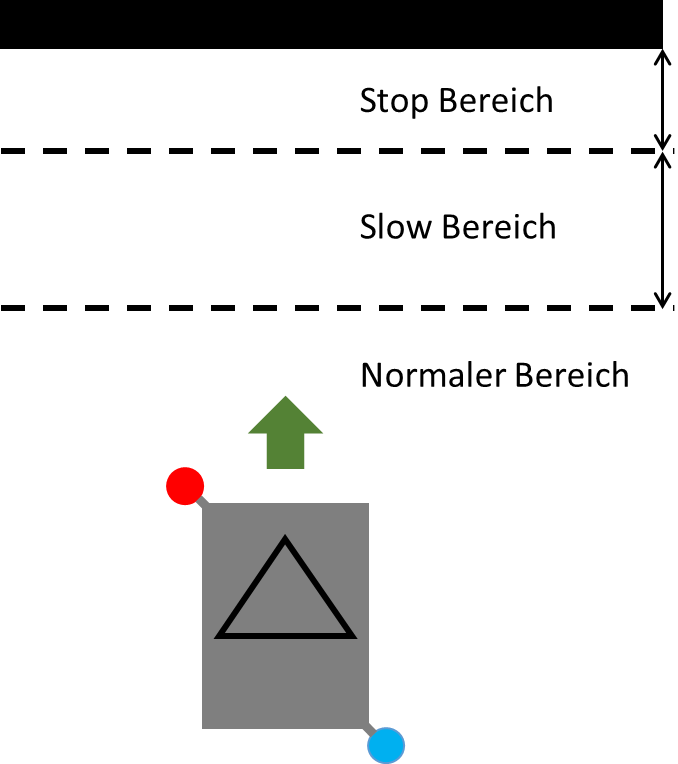
\includegraphics[width=0.6\textwidth]{graphics/Zone.png}
\caption{Defining of various speeds depending on the distance to the obstacle}
\label{Zone}
\centering
\end{figure}

As mentioned before the core of the recovery algorithm is the function \texttt{moveForward()}. Its logic is depicted in Figure \ref{move_forward} and its single steps in the following description:

\begin{figure}[ht]
\centering
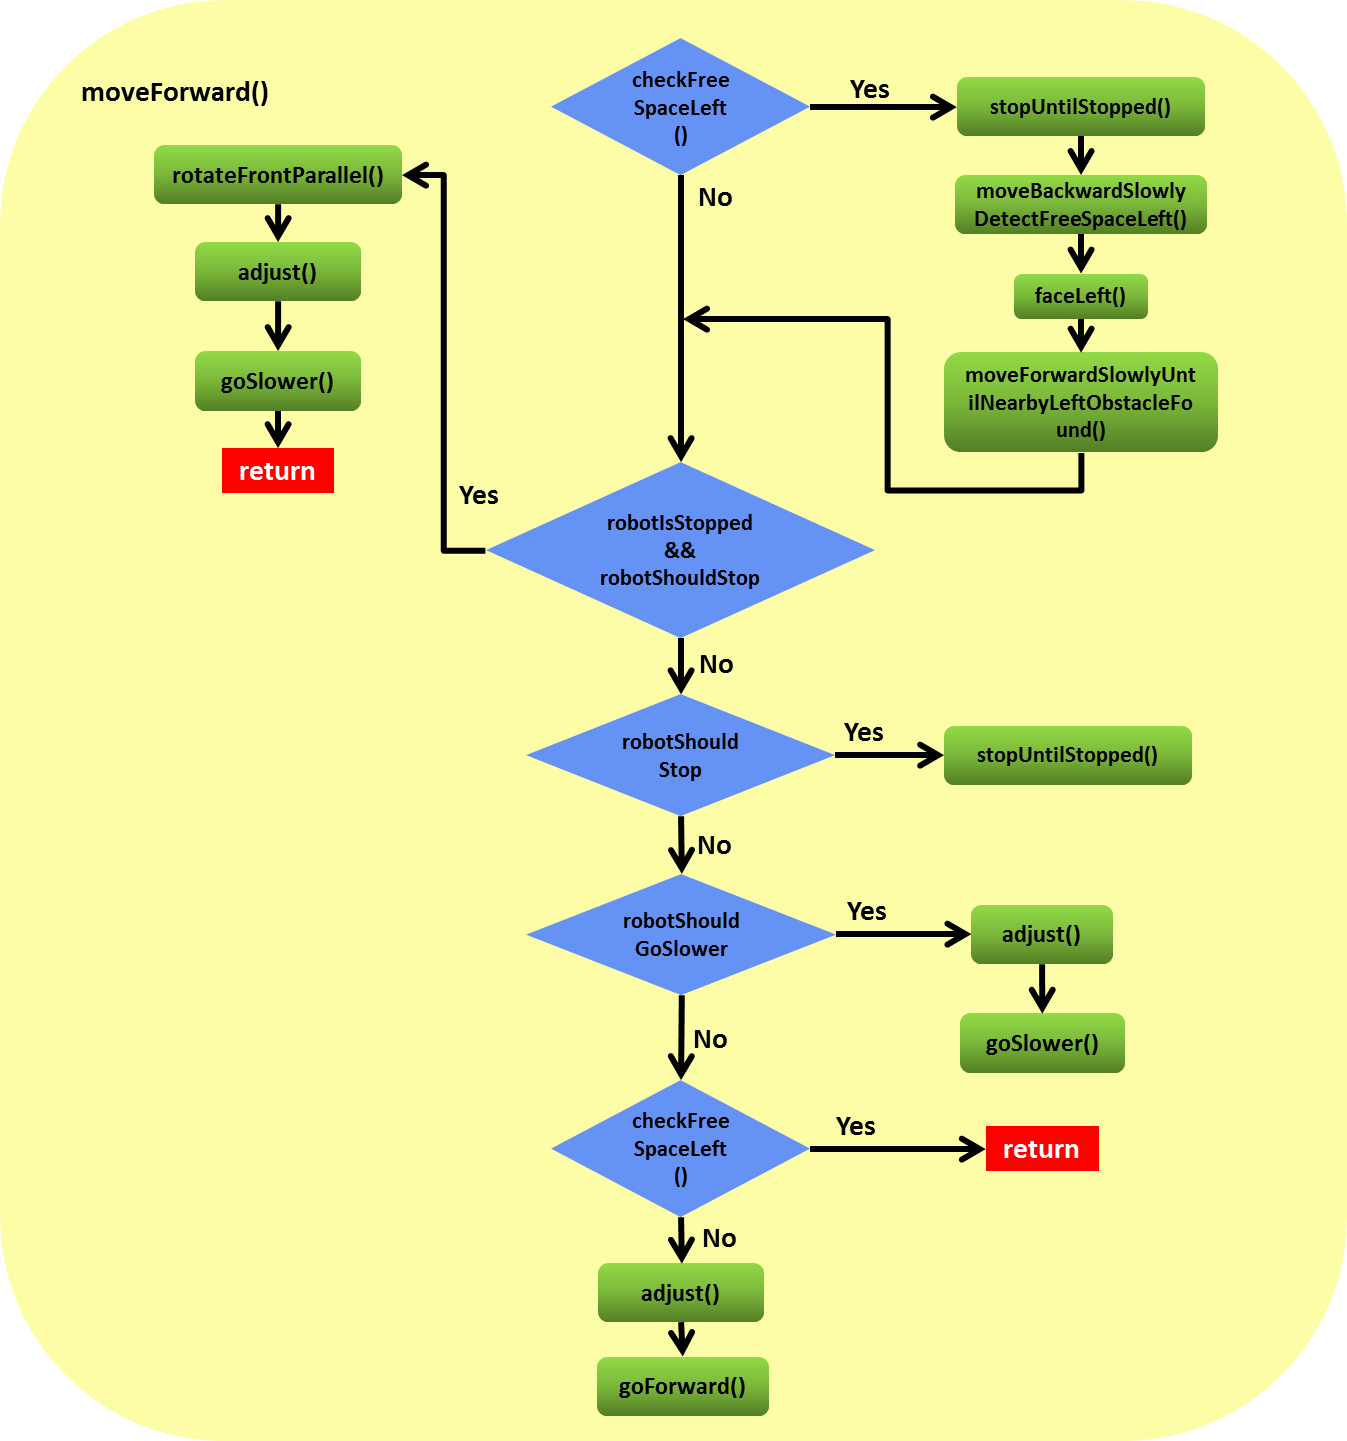
\includegraphics[width=0.9\textwidth]{graphics/move_forward.png}
\caption{Core step of the recovery algorithm}
\label{move_forward}
\centering
\end{figure}

\begin{description}
\item[checkFreeSpaceLeft()] The function checks if there is a free space on the left side of the robot. It is calculated by considering all the points that are located within the left interval, so ``beside'' of the robot. The candidate with minimal distance to the robot is taken and if that is far enough, free space is detected.
\item[stopUntilStopped()] The function stops the robot. It is realized by publishing linear and angular twist of the robot as zero. Because a simple publishing would result in the code to continue its execution, the function waits until the robot really stops. The threshold is set so that a negligibly small value of twist is recognized as zero.
\item[moveBackwardSlowlyDetectFreeSpaceLeft()] The function makes the robot go a few steps back slowly which should compensate its dynamics while it detects the free space on the left. Going backward with velocity  \texttt{-SLOW\_BACKWARD\_VELOCITY} happens until free space is detected and until chosen time \texttt{BACKWARD\_PAUSE} has elapsed. The presence of free space shall be obvious if nothing changed, since it was already detected before.
\item[faceLeft()] The function simply rotates 90$^{\circ}$ counterclockwise so that the robot faces the free space it has detected.
\item[moveForwardSlowlyUntilNearbyLeftObstacleFound()] The function moves the robot slowly forwards until the nearby obstacle is detected there. A blind spot interval in front-left direction is introduced in which points are not considered yet.

The function \texttt{checkObstacleLeftFrontBlindSpot()} checks points in that interval and if there is any obstacle closer than chosen \texttt{FREE\_LEFT\_SPACE\_DISTANCE} it makes the robot rotate 4$^{\circ}$ clockwise, otherwise 8$^{\circ}$ counterclockwise. This solution prevents a situation in which the robot moves on without noticing an obstacle in its blind spot. Different angle values take care of non-ambiguous classification of points located there to one of the other intervals, front or left.
\item[robotIsStopped] The flag indicates if the robot has stopped or not. That depends on the values of linear twist compared to zero in function \texttt{isStopped()}
\item[robotShouldStop] The flag indicates if the robot should stop. This is the case if its current distance to the closest obstacle is not bigger than \texttt{MIN\_CAUTION\_DISTANCE}, which is chosen to be 0.11 meter.
\item[rotateFrontParallel()] The function rotates the robot until it is aligned parallel to the obstacle in its front, as shown in figure \ref{parallel}. Merged information from both front and back lasers is used. Two closest points that are detected in front interval are considered a pair from which an average is calculated. That average is treated as a pivot point for the robot rotation. Points which are detected around the pivot are grouped into either left or right side and averaged again. The resulting final left and right average points form a vector to which the robot has to align itself. The averaging adds robustness to the process and tackles the problem of longitudinal inaccuracy of the laser scans.
\item[adjust()] The function consists of two subtasks: \texttt{rotateLeftParallel()} and \\ \texttt{adjustLeftDistance()}. The first one makes the robot correct its orientation to maintain its left side in parallel manner to the obstacle. The second one makes the robot maintain a proper distance to that obstacle. It must be enough to eventually rotate, but not too much since the maze-algorithm implementation requires the robot to move left along the obstacle. At the same time function \texttt{checkRightObstacle()} checks if there is no obstacle on the immediate right of the robot, so that it can adjust its left distance. To maintain left side parallel a vector is needed to define the corrective rotation, as shown in Figure \ref{rotate_left_parallel02}. Here both merged information from front as well as back lasers are used. It considers those points that are placed on the left side of the robot. Half of them form the left group, another half the right group. The average point is computed for each of both groups and the two points form the needed vector. However the points cannot be placed too far away from each other, as it could indicate another obstacle behind the main one, as shown in Figure \ref{rotate_left_parallel01}. Including such points into average calculation would corrupt the result and deliver an undesired rotation angle.
\item[robotShouldGoSlower()]  The flag indicates if the robot should stop. It is so if its current distance to the closest obstacle is not bigger than \texttt{MIN\_FRONT\_DISTANCE}, chosen to be 0.3 meter. 
\item[goSlower()] The function simply makes the robot go forward with the given velocity \\ \texttt{SLOW\_FORWARD\_VELOCITY}
\item[goForward()] The function simply makes the robot go forward with the given velocity \\ \texttt{DEFAULT\_FORWARD\_VELOCITY} 
\end{description}

\begin{figure}[ht]
\centering
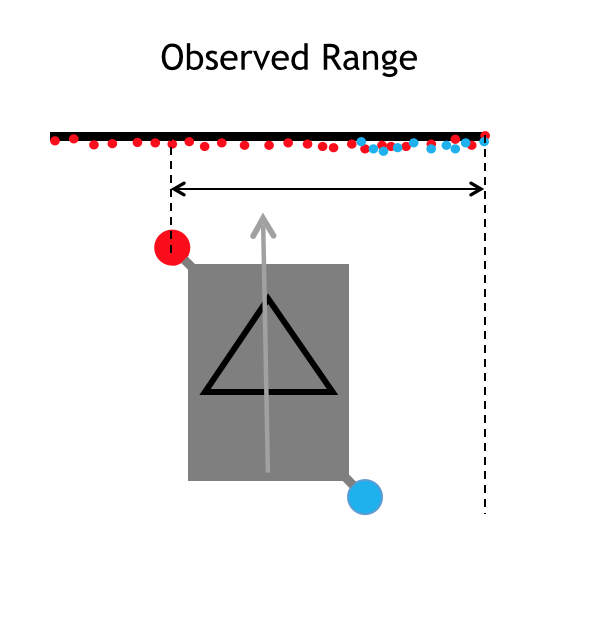
\includegraphics[width=0.5\textwidth]{graphics/betrachteter_bereich.png}
\caption{Considering buffer area on the right}
\label{betrachteter_bereich}
\centering
\end{figure}

\begin{figure}[ht]
\centering
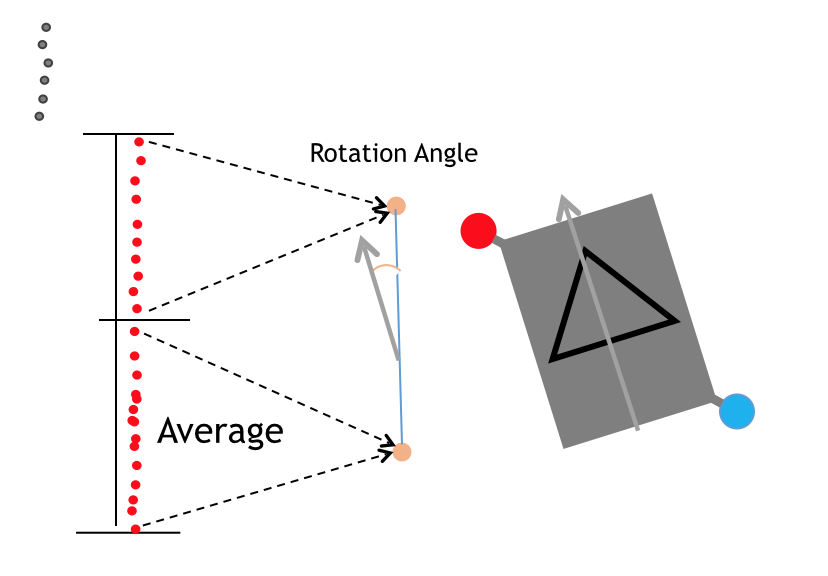
\includegraphics[width=0.7\textwidth]{graphics/rotate_left_parallel02.png}
\caption{Rotating to align left side parallel to the obstacle}
\label{rotate_left_parallel02}
\centering
\end{figure}

\begin{figure}[ht]
\centering
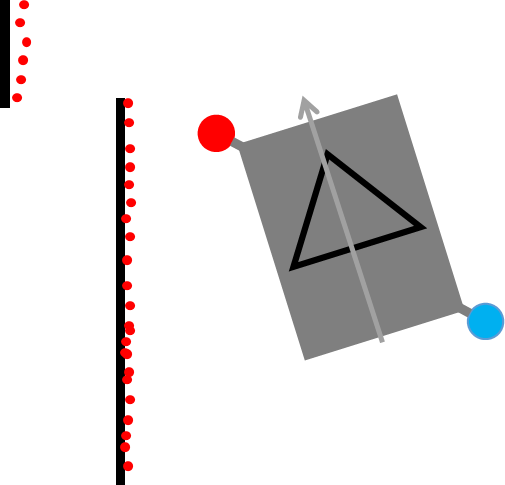
\includegraphics[width=0.6\textwidth]{graphics/rotate_left_parallel01.png}
\caption{Result of obstacle scanning on the left side of the robot}
\label{rotate_left_parallel01}
\centering
\end{figure}

Due to the fact that the maze-solving-algorithm consists of moving on the left side and rotating clockwise, the front of the robot is a bit asymmetric as shown in Figure \ref{betrachteter_bereich}. There is a bit more space on the right to make sure that the robot is able to rotate any time it needs.

\section{Problems and Difficulties} \label{problems}
During our work we encountered various difficulties of the workplace and its environment and we list them in the following subsections.

\subsection{Calibration}
Two laser scanners of the robot turned out to be not calibrated properly. Due to lack of documentation of configuration files we spent a big amount of time searching the proper ones by changing the values and observing the results in rviz. Physical alignment was also needed to keep the right angles with respect to the robot's body. If not calibrated properly, laser sensors would deliver the point clouds which do not represent the obstacles properly. For example boxes placed parallel to the robot would not be parallel in the environment visualization. Wrong calibration could be also easily seen in the areas where the data of front and back sensor overlap. If we put the obstacle in such area and observed points from both sensors that would overlap in rviz we knew that sensors were properly calibrated.

\subsection{Floor Level}
In HoLL there is an inclination in the middle of the corridor. Since the laser sensors operate on one specific height, from a certain point the inclination was detected as an obstacle, just the same as any wall around. To avoid this, the proper interpretation of the distance measure had to be considered.
When the robot was moving downwards and was instructed to stop, its wheels did not stop completely at once and it was actually coasting for some time.

\subsection{Uneven Surface}
Another difficulty for both the robot and for us was the uneven surface. When trying to drive over it or rotate on it, it happened very often that the wheels spinned in the air and the information coming from odometry did not reflect the reality anymore. It produced problems for both rotation and translation actions. Additionally we often encountered situations, in which the robot tried to move forward but couldn't and moved backward  instead due to incorrect odometry values. Consequently, the next information it obtained about obstacles was irrelevant and resulted in a undesired behavior.

\subsection{Transparent Window}
Finally, the transparent office walls in HoLL posed another difficulty. One obvious reason was the danger of destroying them, especially in the initial phase of interaction with the robot and the initial version of the algorithm which we started to test. Secondly, the laser sensors did not recognize glass and delivered point clouds not precise to the position of the windows. To solve this problem we used styrofoams and cardboards which we found in the laboratory to protect the windows and build provisional walls that laser sensors could detect.
